\newcommand{\adag}[1]{\hat{a}_{#1}^\dagger}
\newcommand{\aop}[1]{\hat{a}_{#1\vphantom{\dagger}}}
\chapter{ Theory: background}
\minitoc\

This chapter will cover the elementary concepts required to describe an membrane based optomechanical system in a quantum regime. We will first recall basics on optical field quantization as well describing coherent and squeezed light field, to then turn to the more specific frequency dependent squeezed light field. Secondly, we will cover the mathematical description of a mechanical resonator interacting with a generic coherent optical field, highlighting the differences with the seminal optomechanical system of a mirror on a spring. Finally, we will derive the equations of motions of a membrane based optomechanical system with frequency dependent squeezed optical fields. 

\section{Quantum Optics Concepts}
\subsection{Quantum Description of Light}
We introduce briefly field quantization concepts needed to describe monochromatic field propagation and measurements.

\subsection*{Quantised Electromagnetic Field}
% \the\textwidth

We consider the quantised electromagnetic field in volume $V$. The electric field operator can be expressed in the Heisenberg picture as:
\begin{equation}
\hat{\mathbf{E}}(\mathbf{r}, t) = i \sum_{ \ell} \mathcal{E}_l \left[\hat{a}_{\ell}^{\vphantom{dagger}}\mathbf{f}_{\ell}^{\vphantom{*}}(\mathbf{r})e^{-i\omega_{\ell}t} - \hat{a}_{\ell}^\dagger \mathbf{f}_{\ell}^*(\mathbf{r}) e^{i\omega_{\ell}t}\right]
\end{equation}
where $\mathcal{E}_l = \sqrt{\frac{\hbar \omega_l}{2 \varepsilon_0 V}}$ is the field per photon in mode $\ell$ with $\hbar$ the reduced Planck constant, $\omega_\ell$ the angular frequency of mode $\ell$ and $\varepsilon_0$ the vacuum permittivity, $\mathbf{f}_{\ell}(\mathbf{r})$ are spatial mode functions satisfying orthonormality, and ($\hat{a}_{\ell}^{\vphantom{\dagger}}$, $\hat{a}_{\ell}^{\dagger}$) are the time dependent annihilation and creation operators associated with each mode $\ell$ satisfying the canonical commutation relations
\[
[\hat{a}_{\ell}^{\vphantom{\dagger}}, \hat{a}_{\ell'}^\dagger] = \delta_{\ell \ell'} , \quad
[\hat{a}_{\ell}^{\vphantom{\dagger}}, \hat{a}_{\ell'}^{\vphantom{\dagger}} ] = 0, \quad [\hat{a}_{\ell}^\dagger , \hat{a}_{\ell'}^\dagger ] = 0  
\]
\subsection*{Fock states}
In this description of the optical field, each mode $\ell$ is modeled as a quantum harmonic oscillator with a discrete set of energy eigenstates known as \textit{Fock states} or number states, denoted $\ket{n_\ell}$. These states form an orthonormal basis and satisfy $\hat{n}_{\ell} \ket{n_\ell} = n_\ell \ket{n_\ell}$, where $\hat{n}_{\ell}$ is the number operator defined by
\[
\hat{n}_{\ell} = \hat{a}_{\ell}^\dagger \hat{a}^{\vphantom{\dagger}}_{\ell}.
\]
The action of the creation and annihilation operators on these states is given by
\[
\hat{a}^{\vphantom{\dagger}}_{\ell} \ket{n_\ell} = \sqrt{n_\ell} \ket{n_\ell - 1}, \quad
\hat{a}_{\ell}^\dagger \ket{n_\ell} = \sqrt{n_\ell + 1} \ket{n_\ell + 1}.
\]
They allow transitions between Fock states by lowering or raising the photon number in mode $\ell$ by one unit. The vacuum state $\ket{0_\ell}$ is annihilated by $\hat{a}^{\vphantom{\dagger}}_{\ell}$, satisfying $\hat{a}^{\vphantom{\dagger}}_{\ell} \ket{0_\ell} = 0$. Thus, the Hamiltonian for the electromagnetic field becomes a sum of harmonic oscillator energies:
\begin{equation}
\hat{H} = \sum_\ell \hbar \omega_{\ell} \left( \hat{n}_\ell + \frac{1}{2} \right)
\end{equation}
\subsection*{Quasi monochromatic fields } 
In realistic optical systems such as lasers, the electromagnetic field is rarely perfectly monochromatic. Instead, it exhibits a finite spectral linewidth due to stimulated emission, phase noise, or intentional modulation. These effects cause the amplitude and phase of the optical field to evolve slowly compared to the optical frequency $\omega_\ell$. \\

\noindent As a result, the complex amplitude associated with each mode, typically captured by the Heisenberg-picture annihilation operator $\hat{a}_\ell(t)$, acquires an explicit time dependence beyond the standard fast-oscillating term $e^{-i\omega_\ell t}$. This slow temporal variation reflects the underlying physics: for instance, amplitude or phase modulation, feedback-induced dynamics, or noise processes can all modulate the quantum state in time. Consequently, in the quasi-monochromatic regime, one often separates the field into a rapidly oscillating carrier and a slowly varying envelope encoded in $\hat{a}_\ell(t)$, allowing a spectrally resolved yet temporally adaptive description of the field. \\

\subsection*{Linearization of the optical field: mean field and fluctuations}

We often consider a single spatial mode of the electromagnetic field with optical frequency \(\omega_0\), and assume the presence of a strong coherent field. In this regime, the annihilation operator is decomposed as \(\hat{a}(t) = \bar{\alpha}(t) + \delta\hat{a}(t)\), where \(\bar{\alpha}(t)=\langle \hat{a}(t)\rangle\) is a classical complex amplitude and \(\delta\hat{a}(t)\) represents quantum fluctuations such that \(\langle \delta \hat{a}(t)=0\rangle\).
Linearizing the electric field operator then yields:
\begin{equation}
\begin{aligned}
\hat{\mathbf{E}}(\mathbf{r}, t) 
&= i \, \mathcal{E} \left[ \bar{\alpha}(t)\, \mathbf{f}(\mathbf{r})\, e^{-i \omega_0 t} 
- \bar{\alpha}^*(t)\, \mathbf{f}^*(\mathbf{r})\, e^{i \omega_0 t} \right] \\
&\quad + i \, \mathcal{E} \left[ \delta \hat{a}(t)\, \mathbf{f}(\mathbf{r})\, e^{-i \omega_0 t}
- \delta \hat{a}^\dagger(t)\, \mathbf{f}^*(\mathbf{r})\, e^{i \omega_0 t} \right]
\end{aligned}
\end{equation}

The first line represents the field classical component, involving the coherent amplitude $\bar{\alpha}(t)$, while the second shows the quantum fluctuation term $\delta\hat{a}(t)$. This linearization simplifies the analysis of the field, allowing us to treat the coherent part as a classical field and the fluctuations as a quantum harmonic oscillator. The field Hamiltonian then reduces to a single-mode harmonic oscillator form:
\begin{equation}
\hat{H} = \hbar \omega_0 \left( \delta \hat{a}^\dagger \delta \hat{a} + \frac{1}{2} \right),
\end{equation}
where $\delta \hat{a}$ is the annihilation operator for the fluctuations. The coherent part contributes a constant energy offset, while the fluctuations behave as a quantum harmonic oscillator with frequency $\omega_0$. This Hamiltonian now features an explicit time dependence through the coherent amplitude $\bar{\alpha}(t)$, which can vary slowly compared to the optical frequency.
Importantly, the fluctuation operators retain the canonical bosonic commutation relations:
\[
[\delta \hat{a}(t), \delta \hat{a}^\dagger(t)] = 1, \qquad
[\delta \hat{a}(t), \delta \hat{a}(t)] = 0, \qquad
[\delta \hat{a}^\dagger(t), \delta \hat{a}^\dagger(t)] = 0.
\]
These ensure that the quantized nature of the field is preserved under linearization, with $\delta \hat{a}(t)$ and $\delta \hat{a}^\dagger(t)$ obeying the same algebra as the original field operators. \\

\textbf{Remarks:} 
\begin{itemize}
  \item The linearization procedure is valid when the coherent amplitude $\bar{\alpha}(t)$ is much larger than the quantum fluctuations, i.e., $|\bar{\alpha}(t)| \gg \langle \delta\hat{a}^\dagger \delta\hat{a} \rangle^{1/2}$.
  \item This approach is widely used in quantum optics and optomechanics to simplify the analysis of systems driven by strong classical fields, such as lasers.
  \item The separation into mean field and fluctuations allows us to treat the quantum noise properties independently from the classical dynamics.
  \item The quantum fluctuation operators $\delta\hat{a}(t)$ describe vacuum or squeezed noise, and their statistics determine the ultimate sensitivity limits in measurement schemes.
  \item Linearization is the starting point for deriving quantum Langevin equations and for analyzing noise spectra in optomechanical systems.
\end{itemize}
\subsection*{Quadrature Operators}

To describe the phase space properties of a field mode, we define the Hermitian quadrature operators $\hat{a}_{1}$ and $\hat{a}_{2}$ as
\begin{equation}
  \begin{split}
    \hat{a}_{1} &= \hat{a}^{\vphantom{\dagger}} + \hat{a}^\dagger  \\
    \hat{a}_{2} &= \hat{a}^{\vphantom{\dagger}} - \hat{a}^\dagger
  \end{split}
\end{equation}
More generally we can define arbitrary quadrature operators as 
\begin{align}
  \hat{a}_{\theta} &= e^{i\theta}\hat{a}+ e^{-i\theta}\hat{a}^{\dagger} \notag \\ 
  & = \cos \theta \hat{a}_{1} + \sin \theta \hat{a}_{2}
\end{align}
where we notice that $\hat{a}_{1} = \hat{a}_{\theta=0\vphantom{\pi/2}}$ and $\hat{a}_{1} = \hat{a}_{\theta=\pi/2}$. These are Hermitian operators corresponding to measurable observables and satisfy the commutation relation
\begin{equation}
[a_{\theta \vphantom{\pi/2}}, a_{\theta+\pi/2}] = 2i
\end{equation}

\subsection*{Uncertainty Principle and Quantum Noise}

For two generic Hermitian operators $\hat{A}$ and $\hat{B}$, the Heisenberg uncertainty principle reads as 
\begin{equation}
  \Delta \hat{A}\Delta \hat{B} \geq \frac{1}{2} |[\hat{A}, \hat{B}]|
\end{equation}
where we defines $\Delta \hat{A}=\sqrt{|\langle \hat{A}^2\rangle - \langle \hat{A} \rangle^2|}$. This defines the minimum amount of quantum noise (vacuum fluctuations) in the electromagnetic field.
Applying this equation to the quadratures defined above we get 
\begin{equation}
   \begin{split}
    \Delta \hat{a}_{1} \Delta \hat{a}_{2} &\geq 1 \\
    \Delta \hat{a}_{\theta \vphantom{\pi/2}} \Delta \hat{a}_{\theta +\pi/2} &\geq 1
   \end{split}
\end{equation}
\subsection*{Coherent States}


\begin{figure}
\centering
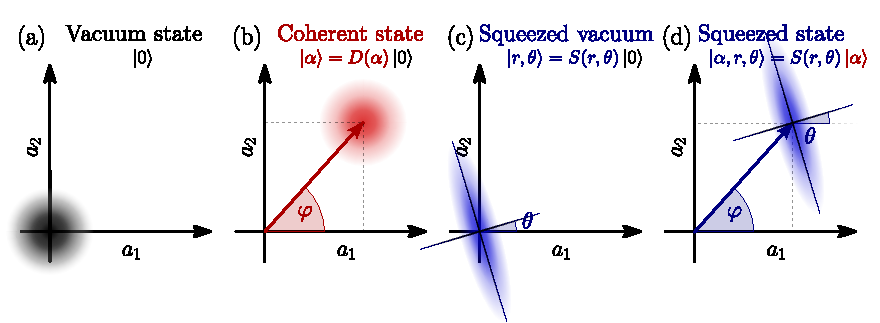
\includegraphics[width=\textwidth]{./chap2/fig/quantumstates (2).pdf}
\caption{Phase-space representations of quantum states and transformations.
(a) Wigner function of the vacuum state: a circular Gaussian centered at the origin, representing equal quantum fluctuations in both quadratures $a_1$ and $a_2$.
(b) Wigner function of a coherent state: a displaced circular Gaussian, showing a shift in phase space along an angle $\varphi$ with unchanged, isotropic noise.
(c) Wigner function of a squeezed vacuum state: an elliptical Gaussian centered at the origin, with reduced noise along a rotated quadrature $X_\theta$ and increased noise in the orthogonal direction.
(d) Wigner function of a displaced squeezed state: an ellipse shifted away from the origin, combining anisotropic fluctuations and a nonzero mean amplitude. The displacement angle $\varphi$ and squeezing angle $\theta$ are independent.} 
\end{figure}

\begin{figure}
\centering
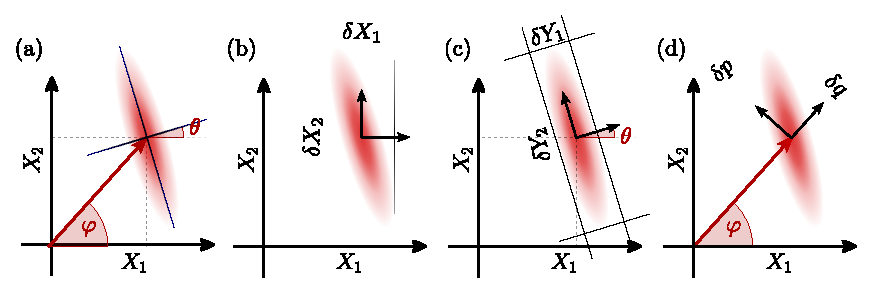
\includegraphics[width=\textwidth]{./chap2/fig/quadratures_phasespace.pdf}
\caption{Phase-space representations of quantum states and transformations.
(a) Wigner function of the vacuum state: a circular Gaussian centered at the origin, representing equal quantum fluctuations in both quadratures $X_1$ and $X_2$.
(b) Wigner function of a coherent state: a displaced circular Gaussian, showing a shift in phase space along an angle $\varphi$ with unchanged, isotropic noise.
(c) Wigner function of a squeezed vacuum state: an elliptical Gaussian centered at the origin, with reduced noise along a rotated quadrature $X_\theta$ and increased noise in the orthogonal direction.
(d) Wigner function of a displaced squeezed state: an ellipse shifted away from the origin, combining anisotropic fluctuations and a nonzero mean amplitude. The displacement angle $\varphi$ and squeezing angle $\theta$ are independent.} 
\end{figure}


We now turn to standard optical quantum states, in particular gaussian states i.e.\ full positive in Wigner functin representations such as coherent and squeezed states, that we will denote in braket notation as $\alpha\rangle$ and  $|\alpha\rangle$ are eigenstates of the annihilation operator:
\begin{equation}
\hat{a}|\alpha\rangle = \alpha|\alpha\rangle
\end{equation}
They can be generated by displacing the vacuum:
\begin{equation}
|\alpha\rangle = \hat{D}|0\rangle, \quad \hat{D}(\alpha) = \exp(\alpha \hat{a}^\dagger - \alpha^* \hat{a})
\end{equation}
They exhibit:
\begin{itemize}
  \item Minimum uncertainty: $\Delta q = \Delta p = 1/\sqrt{2}$
  \item Classical-like dynamics
  \item Poissonian photon statistics
\end{itemize}

\subsection*{Squeezed States}

Squeezed states reduce the variance of one quadrature below vacuum level:
\begin{align}
|\xi_{\omega,\ell}\rangle &= \hat{S}(\xi_{\omega,\ell}) |0\rangle \\
\hat{S}(\xi) &= \exp\left[\frac{1}{2}(\xi^* \hat{a}^2 - \xi \hat{a}^{\dagger 2})\right], \quad \xi = r e^{i\phi}
\end{align}
For phase quadrature squeezing ($\phi = 0$):
\begin{equation}
\Delta q_{\omega,\ell} = e^{-r}/\sqrt{2}, \quad \Delta p_{\omega,\ell} = e^{r}/\sqrt{2}
\end{equation}
Squeezed light is a key resource for precision metrology and quantum information.


\vspace{1em}
This concludes our introduction to the quantum description of light, setting the stage for modelling interactions between quantum optical fields and mechanical resonators.

\subsection{\textcolor{red}{Optical Field Modulations}}
\subsubsection*{Linearization of the Electric Field and Modulation Sidebands}

We consider a single optical mode with a strong coherent drive. The annihilation operator is linearized as:
\begin{equation}
    \hat{a}(t) \to \bar{\alpha}(t) + \delta \hat{a}(t)
\end{equation}
where $\bar{\alpha}(t) \in \mathbb{C}$ is the classical coherent amplitude and $\delta \hat{a}(t)$ captures quantum fluctuations.

The classical part of the electric field is then:
\begin{equation}
    \mathbf{E}_{\text{cl}}(\mathbf{r}, t) = i \sqrt{\frac{\hbar \omega}{2 \varepsilon_0}} \left[
    \mathbf{f}(\mathbf{r})\, \bar{\alpha}(t)\, e^{-i \omega t}
    - \mathbf{f}^*(\mathbf{r})\, \bar{\alpha}^*(t)\, e^{i \omega t}
    \right]
\end{equation}

We now consider two types of sinusoidal modulation at frequency $\Omega$:

\subsubsection*{Amplitude Modulation (AM)}

Let the coherent amplitude be modulated in amplitude:
\begin{equation}
    \bar{\alpha}(t) = \bar{\alpha}_0 \left(1 + \epsilon_a \cos(\Omega t)\right)
    = \bar{\alpha}_0 \left(1 + \frac{\epsilon_a}{2} e^{i\Omega t} + \frac{\epsilon_a}{2} e^{-i\Omega t} \right)
\end{equation}
with $\epsilon_a \ll 1$. The conjugate is:
\begin{equation}
    \bar{\alpha}^*(t) = \bar{\alpha}_0^* \left(1 + \frac{\epsilon_a}{2} e^{i\Omega t} + \frac{\epsilon_a}{2} e^{-i\Omega t} \right)
\end{equation}

Substituting into the field expression:
\begin{align}
    \mathbf{E}_{\text{cl}}^{\text{(AM)}}(\mathbf{r}, t) =
    i \sqrt{\frac{\hbar \omega}{2 \varepsilon_0}} \Big[
    &\mathbf{f}(\mathbf{r})\, \bar{\alpha}_0 \left( e^{-i\omega t} + \frac{\epsilon_a}{2} e^{-i(\omega - \Omega)t} + \frac{\epsilon_a}{2} e^{-i(\omega + \Omega)t} \right) \nonumber \\
    - &\mathbf{f}^*(\mathbf{r})\, \bar{\alpha}_0^* \left( e^{i\omega t} + \frac{\epsilon_a}{2} e^{i(\omega - \Omega)t} + \frac{\epsilon_a}{2} e^{i(\omega + \Omega)t} \right)
    \Big]
\end{align}

\subsubsection*{Phase Modulation (PM)}

Now consider phase modulation of the coherent amplitude:
\begin{equation}
    \bar{\alpha}(t) = \bar{\alpha}_0 e^{i \epsilon_\phi \cos(\Omega t)}
    \approx \bar{\alpha}_0 \left(1 + i \epsilon_\phi \cos(\Omega t)\right)
    = \bar{\alpha}_0 \left(1 + \frac{i \epsilon_\phi}{2} e^{i\Omega t} + \frac{i \epsilon_\phi}{2} e^{-i\Omega t} \right)
\end{equation}
and
\begin{equation}
    \bar{\alpha}^*(t) \approx \bar{\alpha}_0^* \left(1 - \frac{i \epsilon_\phi}{2} e^{i\Omega t} - \frac{i \epsilon_\phi}{2} e^{-i\Omega t} \right)
\end{equation}

Substituting into the field:
\begin{align}
    \mathbf{E}_{\text{cl}}^{\text{(PM)}}(\mathbf{r}, t) =
    i \sqrt{\frac{\hbar \omega}{2 \varepsilon_0}} \Big[
    &\mathbf{f}(\mathbf{r})\, \bar{\alpha}_0 \left( e^{-i\omega t} + \frac{i \epsilon_\phi}{2} e^{-i(\omega - \Omega)t} + \frac{i \epsilon_\phi}{2} e^{-i(\omega + \Omega)t} \right) \nonumber \\
    - &\mathbf{f}^*(\mathbf{r})\, \bar{\alpha}_0^* \left( e^{i\omega t} - \frac{i \epsilon_\phi}{2} e^{i(\omega - \Omega)t} - \frac{i \epsilon_\phi}{2} e^{i(\omega + \Omega)t} \right)
    \Big]
\end{align}

\subsection*{Interpretation}

In both cases, the field contains a carrier at frequency $\omega$ and two sidebands at $\omega \pm \Omega$. Amplitude modulation results in sidebands that are in phase with the carrier, while phase modulation produces sidebands with a $\pm \pi/2$ phase shift relative to the carrier.

\subsection{Quantum Noise and Uncertainty}
\subsection{Sideband Representation}
\hspace{1pt}

\section{Optical Cavities: Basics}
\subsection{Cavity types and Resonance Conditions}
\subsection{Spatial and Longitudinal Modes}
\subsection{Static and Dynamical effects}
\hspace{1pt}

\section{\texorpdfstring{\color{red}Optical Cavities: Three Mirror Cavities}{Optical Cavities: Three Mirror Cavities}}
\subsection{}
\hspace{1pt}

\section{Cavity Optomechanics}
\subsection{Radiation Pressure Coupling}
\subsection{Quantum Langevin Equations}
\subsection{\texorpdfstring{Mechanical Resonators}{Mechanical Resonators}}
\subsection{Noise spectra}
\subsection{\texorpdfstring{\color{red} Three Mirror Cavities as Novel Optomechanical Systems}{Three Mirror Cavities as Novel Optomechanical Systems}}
\hspace{1pt}

\section{Squeezed Light Theory}
\subsection{Single-mode Squeezing}
\subsection{Noise Spectra }
\subsection{Frequency-dependent Squeezing and its use}
\hspace{1pt}

\section{Numerical Methods and Simulations}

lets write smth here 
